\documentclass[a4paper,11pt]{article}
\title{PAG 9.1 Charging and discharging capacitors (iii) writeup}
\author{Izaak van Dongen}

% so the title can be accessed by fancyhdr (and is automatically correctly
% spelled etc)
\makeatletter
\let\thetitle\@title
\makeatother

% fonts
\usepackage[p,osf]{cochineal}
\usepackage[scale=.95,type1]{cabin}
\usepackage[cochineal,bigdelims,cmintegrals,vvarbb]{newtxmath}
% fixed width font with 80 chars per listing line
\usepackage[scaled=.94]{newtxtt}
\usepackage[cal=boondoxo]{mathalfa}

% make the document take up more of the page
\usepackage[margin=1in,headheight=13.6pt]{geometry}

% no paragraph indent
\usepackage[parfill]{parskip}

% custom document header/footer
\usepackage{fancyhdr}
\usepackage{lastpage}

\pagestyle{fancy}
\fancyhf{}
\lhead{\thetitle}
\rhead{Izaak van Dongen}
\rfoot{Page \thepage\ of \pageref{LastPage}}

% pretty table rules and multirow entries. Also page-breaking tables
\usepackage{booktabs}
\usepackage{multirow}
\usepackage{longtable}

% plotting mathematical functions (needs version request)
\usepackage{pgfplots}
\pgfplotsset{compat=1.15}

% \url function and clickable table of contents. no ugly red boxes though
\usepackage[hidelinks]{hyperref}

% maths symbols and other stuff (supersedes the ams* packages)
\usepackage{mathtools}

% For framing definitions
\usepackage[framemethod=tikz]{mdframed}
\usepackage[most]{tcolorbox}

\newtcolorbox{definition}{
freelance,
before=\par\vspace{2\bigskipamount}\noindent,
after=\par\bigskip,
frame code={
  \node[
  anchor=south west,
  inner xsep=8pt,
  xshift=8pt,
  rounded corners=5pt,
  font=\bfseries\color{white},
  fill=gray] at (frame.north west) (tit) {\strut Definition:};
  \draw[
  line width=3pt,
  rounded corners=5pt,gray
  ] (tit.west) -| (frame.south west) -- ([xshift=15pt]frame.south west);
},
interior code={},
top=2pt
}

% for better table of contents stuff, providing the \listof* commands and not
% listing the tables in the table of contents
\usepackage[nottoc,notlof,notlot]{tocbibind}

% more advanced handling of utf8 and fonts or something. apparently good to have
\usepackage[utf8]{inputenc}
\usepackage[T1]{fontenc}

% bibliography management with square braces for citations
\usepackage[square,numbers]{natbib}

% graphics, like eps files and stuff (supersedes graphics)
\usepackage{graphicx}

% used to horizontally align floats
\usepackage{subfig}

% used for figures
\usepackage{float}

% needed for colouring and stuff (xcolor supersedes color)
\usepackage{xcolor}

\definecolor{codegreen}{rgb}{ 0,0.6,0}

% listings of code
\usepackage{minted}
\setminted{breaklines,
           breakbytokenanywhere,
           linenos
}
\usemintedstyle{friendly}
% bigger line numbers
\renewcommand\theFancyVerbLine{\footnotesize\arabic{FancyVerbLine}}

% that can break across pages while being captioned figures
\usepackage{caption}
\newenvironment{longlisting}
{\addvspace{\baselineskip}\captionsetup{type=listing}}
{\addvspace{\baselineskip}}

% allow maths to break across pages
\allowdisplaybreaks

\usepackage{csvsimple}
\usepackage{siunitx}

\begin{document}
    \maketitle%\thispagestyle{empty} % no page number under title

\begin{table}[h]
\begin{center}
\begin{tabular}{r S S S S S}
    \toprule
    t / \si{\second} & \multicolumn{5}{c}{I / \si{\ampere}} \\
    \cmidrule(l){2-6} & 1 & 2 & 3 & 4 & 5 \\
    \midrule
    \csvreader[no head]{data.csv}{}
    {\csvcoli&\csvcolii&\csvcoliii&\csvcoliv&\csvcolv&\csvcolvi\\}
\end{tabular}
\end{center}
\caption{Discharging data}
\end{table}

\begin{longlisting}
\inputminted{R}{analyse.r}
\caption{R source}
\end{longlisting}

\begin{figure}[h]
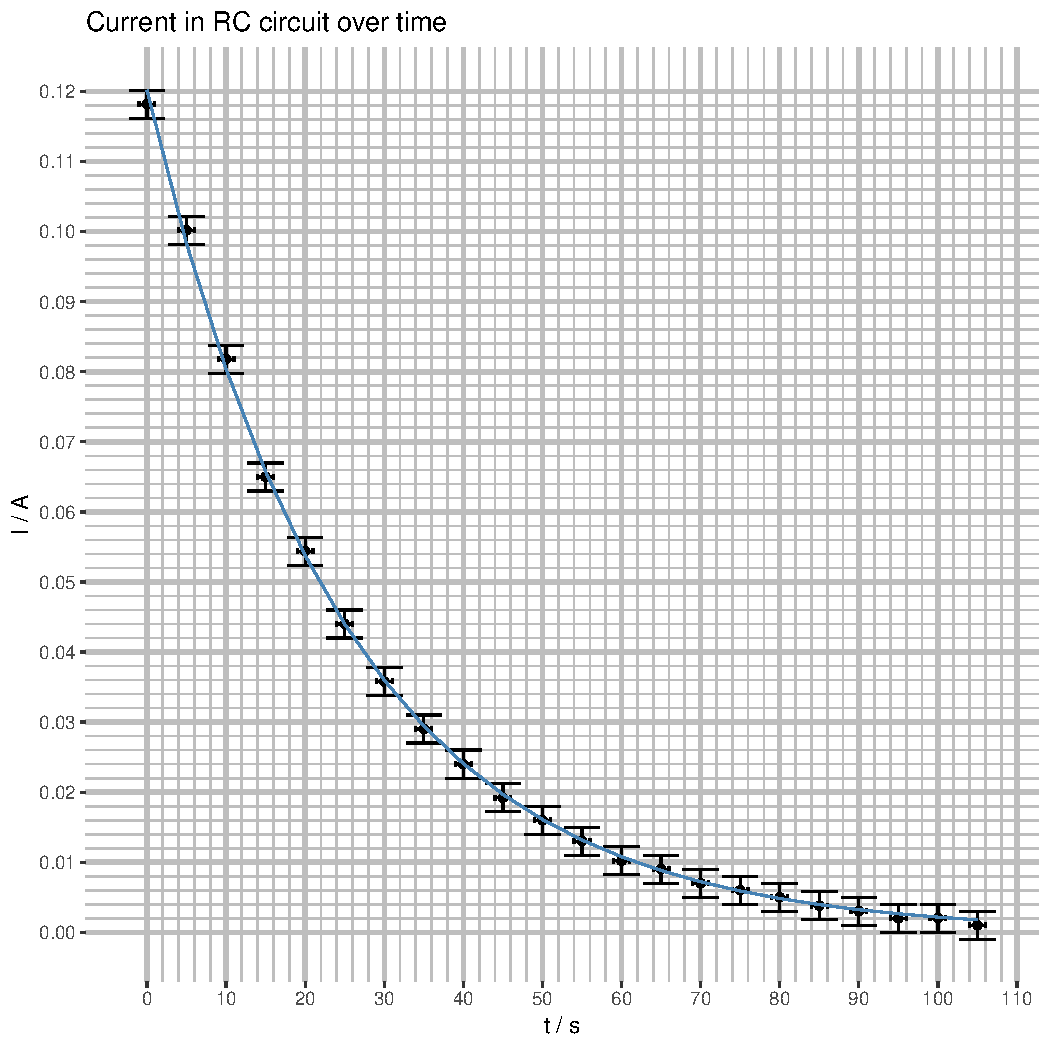
\includegraphics[width=\textwidth]{Rplots.pdf}
\caption{Generated graph}
\end{figure}

\begin{longlisting}
\begin{minted}{text}
Nonlinear regression model
  model: I_avg ~ I0 * exp(-t/tau)
   data: charge_df
     I0     tau
 0.1202 24.8685
 residual sum-of-squares: 1.25e-05

Number of iterations to convergence: 3
Achieved convergence tolerance: 9.243e-07
\end{minted}
\caption{Model results}
\end{longlisting}

The resistance was also measured at \si{47\kilo\ohm}. This can be combined with
the fitted value $\tau = \SI{24.8685}{\second}$, to find

\begin{math}
C = \frac{RC}{R} = \frac{24.8685}{47 \cdot 10^3} = \SI{5.2911e-4}{\farad}
\end{math}

\end{document}
